\documentclass[slidestop]{beamer}
\usepackage{beamerthemesplit}
\usepackage{graphics}
\usepackage{pstricks}

\title{Pin Multiplexer}
\author{Rishabh Jain}
\author{Luke Kenneth Casson Leighton}


\begin{document}

\frame{
   \begin{center}
    \huge{Pin Multiplexer}\\
    \vspace{32pt}
    \Large{Auto-generating documentation, code \\
			and resources for a Pinmux}\\
    \vspace{16pt}
    \Large{Saving time and money for SoC / EC designers\\
		    in the RISC-V Ecosystem and beyond}\\
    \vspace{24pt}
    \Large{[proposed for] Chennai 9th RISC-V Workshop}\\
    \vspace{16pt}
    \large{\today}
  \end{center}
}


\frame{\frametitle{Credits and Acknowledgements}

 \begin{itemize}
   \item TODO\vspace{10pt}
  \end{itemize}
}


\frame{\frametitle{Glossary}

 \begin{itemize}
   \item GPIO: general-purpose reconfigureable I/O (Input/Output).
   \item Pin: an I/O pad.  May be driven (input) or may drive (output).
   \item FN: term for a single-wire "function", such as UART\_TX,
	     I2C\_SDA, SDMMC\_D0 etc.  may be an input, output or both
		 (bi-directional case: two wires are {\bf always} allocated, one
		  for input to the function and one for output from the function).
   \item Bus: a group of bi-directional functions (SDMMC D0 to D3)
         where the direction is ganged and {\bf under the Bus's control}
   \item Input Priority Muxer: a multiplexer with N selector
		 wires and N associated inputs.  The lowest (highest?) indexed
		 "selector" enabled results in its 
		 input being routed to the output.
   \item Output Muxer: a many-to-one "redirector" where any one
	     output "routed" to the input, based on a selector "address".
  \end{itemize}
}


\frame{\frametitle{Why, How and What is a Pinmux?}

 \begin{itemize}
   \item Why? To save cost, increase yield, and to target multiple
         markets with the same design, thereby increasing uptake
         and consequently taking advantage of volume pricing.\vspace{4pt}
         \\
         Summary: it's all about making more money!\vspace{4pt}
   \item How? By multiplexing many more functions (100 to 1,200) than there
         are actual available pins (48 to 500), the required chip package
	     is far less costly and the chip more desirable\vspace{4pt}
   \item What? A many-to-many dynamically-configureable router of
         I/O functions to I/O pins\vspace{4pt}
   \item \bf{Note: actual muxing is deceptively simple, but like
         a DRAM cell it's actually about the ancillaries / extras}
  \end{itemize}
}


\frame{\frametitle{Associated Extras}

 \begin{itemize}
   \item Design Specification
   \item Scenario analysis (whether the chip will fit "markets")
   \item Documentation: Summary sheet, Technical Reference Manual.
   \item Test suites
   \item Control Interface (AXI4 / Wishbone / TileLink / other)
   \item Simulation
   \item Linux kernel drivers, DTB, libopencm3, Arduino libraries etc.
  \end{itemize}
 Example context:
 \begin{itemize}
   \item Shakti M-Class has 160 pins with a 99.5\% full 4-way mux
   \item Almost 640-way routing, 6 "scenarios" (7th TBD),
         100+ page Manual needed,
         \bf{17,500 lines of auto-generated code}
  \end{itemize}
}


\frame{
  \vspace{30pt}
  \begin{center}
    {\Huge 
		   ALL of these\vspace{20pt}\\
		   can be\vspace{20pt}\\
		   auto-generated\vspace{30pt}
	}
	\\
	(from the Design Specification, after Scenario Analysis)
  \end{center}
  
}

\frame{\frametitle{Reduce workload, reduce duplication, reduce risk and cost}

 \begin{itemize}
   \item Auto-generate everything: documentation, code, libraries etc.
	     \vspace{10pt}
   \item Standardise: similar to PLIC, propose GPIO and Pinmux\\
	     saves engineering effort, design effort and much more
	     \vspace{10pt}
   \item Standardise format of configuration registers:
	     saves code duplication effort (multiple software environments)
		 \vspace{10pt}
   \item Add support for multiple code formats: Chisel3 (SiFive IOF),
	     BSV (Bluespec), Verilog, VHDL, MyHDL.
		 \vspace{10pt}
   \item Multiple auto-generated code-formats permits cross-validation:\\
	     auto-generated test suite in one HDL can validate a muxer
	     generated for a different target HDL.
   		 \vspace{10pt}
  \end{itemize}
}


\frame{\frametitle{Design Spec and Scenario Analysis}

 \begin{itemize}
   \item Analyse the target markets that the chip will sell in\\
	     (multiple markets increases sales volume, reduces chip cost)
	     \vspace{4pt}
   \item Create a formal (python-based) specification for the pinmux
	     \vspace{4pt}
   \item Add scenarios then check that they meet the requirements\\
	     { \bf (before spending money on hardware engineers!) }
	     \vspace{4pt}
   \item Scenarios represent target markets: ICs to be connected\\
         (GPS, NAND IC, WIFI etc.  May require draft schematics
         drawn up, or client-supplied schematics analysed).
		 \vspace{4pt}
   \item Analyse the scenarios: if pins are missing, alter and repeat.\\
		 \vspace{4pt}
   \item Eventually the pinmux meets all requirements...\\
	     { \bf without spending USD \$5-50m to find out it doesn't!}
  \end{itemize}
}



\frame{\frametitle{Example: 7 banks, 4-way mux, 160 pins}
 \begin{center}
  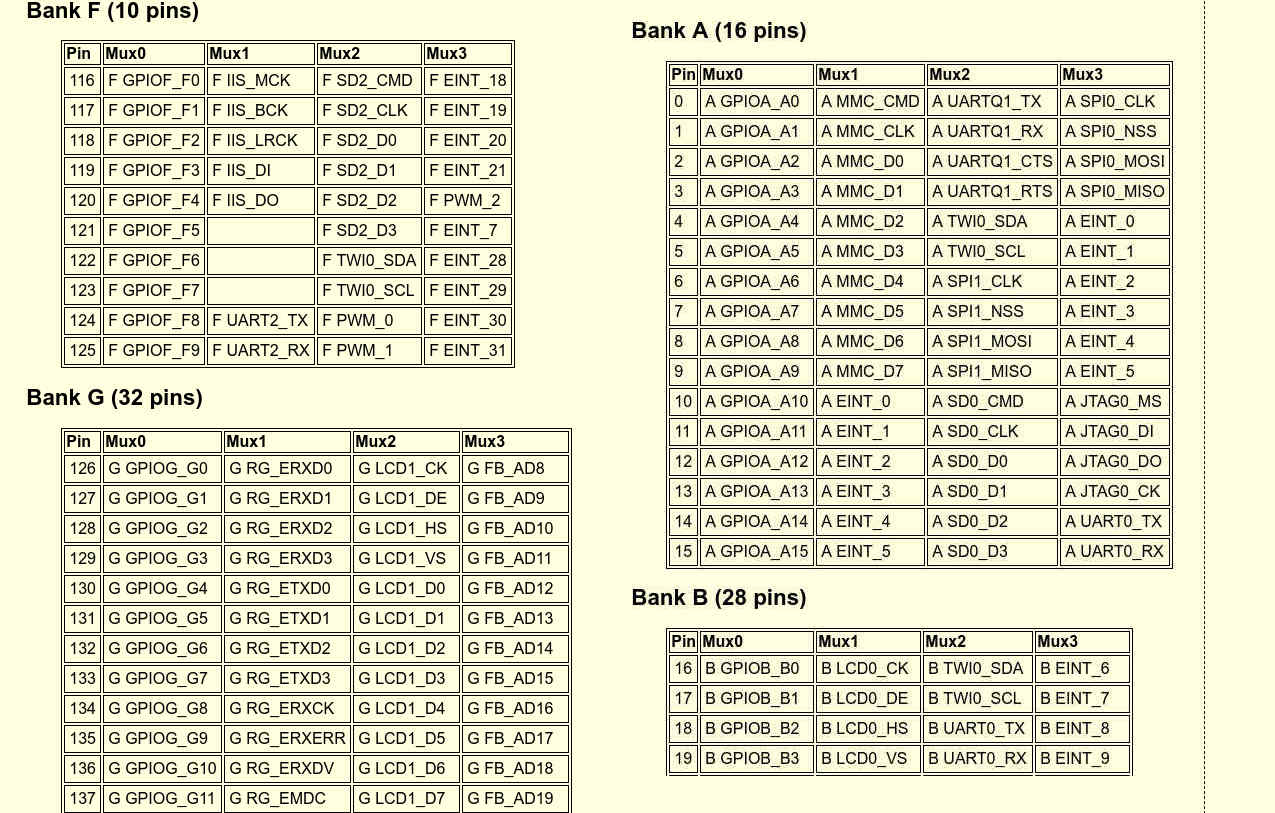
\includegraphics[height=1.7in]{example_pinmux.jpg}
 \end{center}
 \begin{itemize}
   \item { \bf 17,500 lines of auto-generated HDL (and climbing)}
   \item { \bf 12,500 lines of auto-generated Summary/Analysis}
   \item Technical Reference Manual expected to be 100+ pages
 \end{itemize}
}


\frame{\frametitle{Muxer cases to handle (One/Many to One/Many) etc.}

 \begin{itemize}
   \item One FN outputs to Many Pins: no problem\\
	     (weird configuration by end-user, but no damage to ASIC)
   \item One Pin to Many FN inputs: no problem\\
         (weird configuration by end-user, but no damage to ASIC)
   \item Many Pins to One FN input: {\bf Priority Mux needed}\\
	     No priority mux: Pin1 = HI, Pin0 = LO, ASIC is damaged
   \item Many FN outputs simultaneously to one Pin: {\bf does not occur}\\
	     (not desirable and not possible, as part of the pinmux design)
   \item Some FNs (I2C\_SDA, SD\_D0..3) are I/O Buses\\
	     Bi-directional control of the Pin must be handed to the
	     FN
   \item Nice to have: Bus sets pintype, signal strength etc.\\
	     e.g. selecting SD/MMC doesn't need manual pin-config.\\
	     \bf{caveat: get that wrong and the ASIC can't be sold}
  \end{itemize}
}


\frame{\frametitle{Pin Configuration, input and output}

 In/out: {\bf Note: these all require multiplexing }
 \begin{itemize}
   \item Output-Enable (aka Input disable): switches pad to In or Out
   \item Output (actually an input wire controlling pin's level, HI/LO)
   \item Input (actually an output wire set based on pin's driven level)
 \end{itemize}
 Characteristics: {\bf Note: these do not require multiplexing }
 \begin{itemize}
   \item Output current level: 10mA / 20mA / 30mA / 40mA
   \item Input hysteresis: low / middle / high. Stops signal noise
   \item Pin characteristics: CMOS Push-Push / Open-Drain
   \item Pull-up enable: built-in 10k (50k?) resistor
   \item Pull-down enable: built-in 10k (50k?) resistor
   \item Muxing and IRQ Edge-detection not part of the I/O pin
   \item Other? (impedance? not normally part of commercial pinmux)
  \end{itemize}
}


\frame{\frametitle{Standard GPIO 4-way in/out Mux and I/O pad}
 \begin{center}
  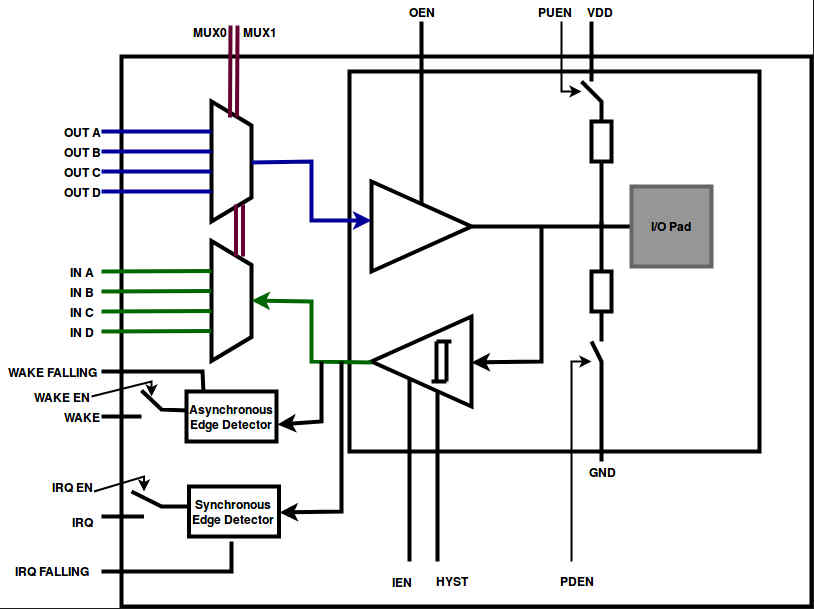
\includegraphics[height=2.5in]{../shakti/m_class/mygpiomux.jpg}\\
  {\bf 4-in, 4-out, pullup/down, hysteresis, edge-detection (EINT)}
 \end{center}
}

\frame{\frametitle{Separating Pin Configuration, input and output}

 \begin{itemize}
   \item Standard Mux design {\bf cannot deal with many-to-one inputs}\\
	     (SiFive IOF source code from Freedom U310 cannot, either)
	     \vspace{4pt}
   \item I/O pad configuration conflated with In-Muxer conflated with
		 Out-Muxer conflated with GPIO conflated with EINT.
         	     \vspace{4pt}
 \end{itemize}
   {\bf IMPORTANT to separate all of these out:
            	     \vspace{4pt}}
 \begin{itemize}
   \item EINTs to be totally separate FNs. managed by RISC-V PLIC\\
         (If every GPIO was an EINT it would mean 100+ IRQs)
            	     \vspace{4pt}
   \item GPIO In/Out/Direction treated just like any other FN\\
	     (but happen to have AXI4 - or other - memory-mapping)
            	     \vspace{4pt}
   \item Pad configuration separated and given one-to-one Registers\\
	     (SRAMs set by AXI4 to control mux, pullup, current etc.)
 \end{itemize}
}

\frame{\frametitle{Register-to-pad "control" settings}
 \begin{center}
  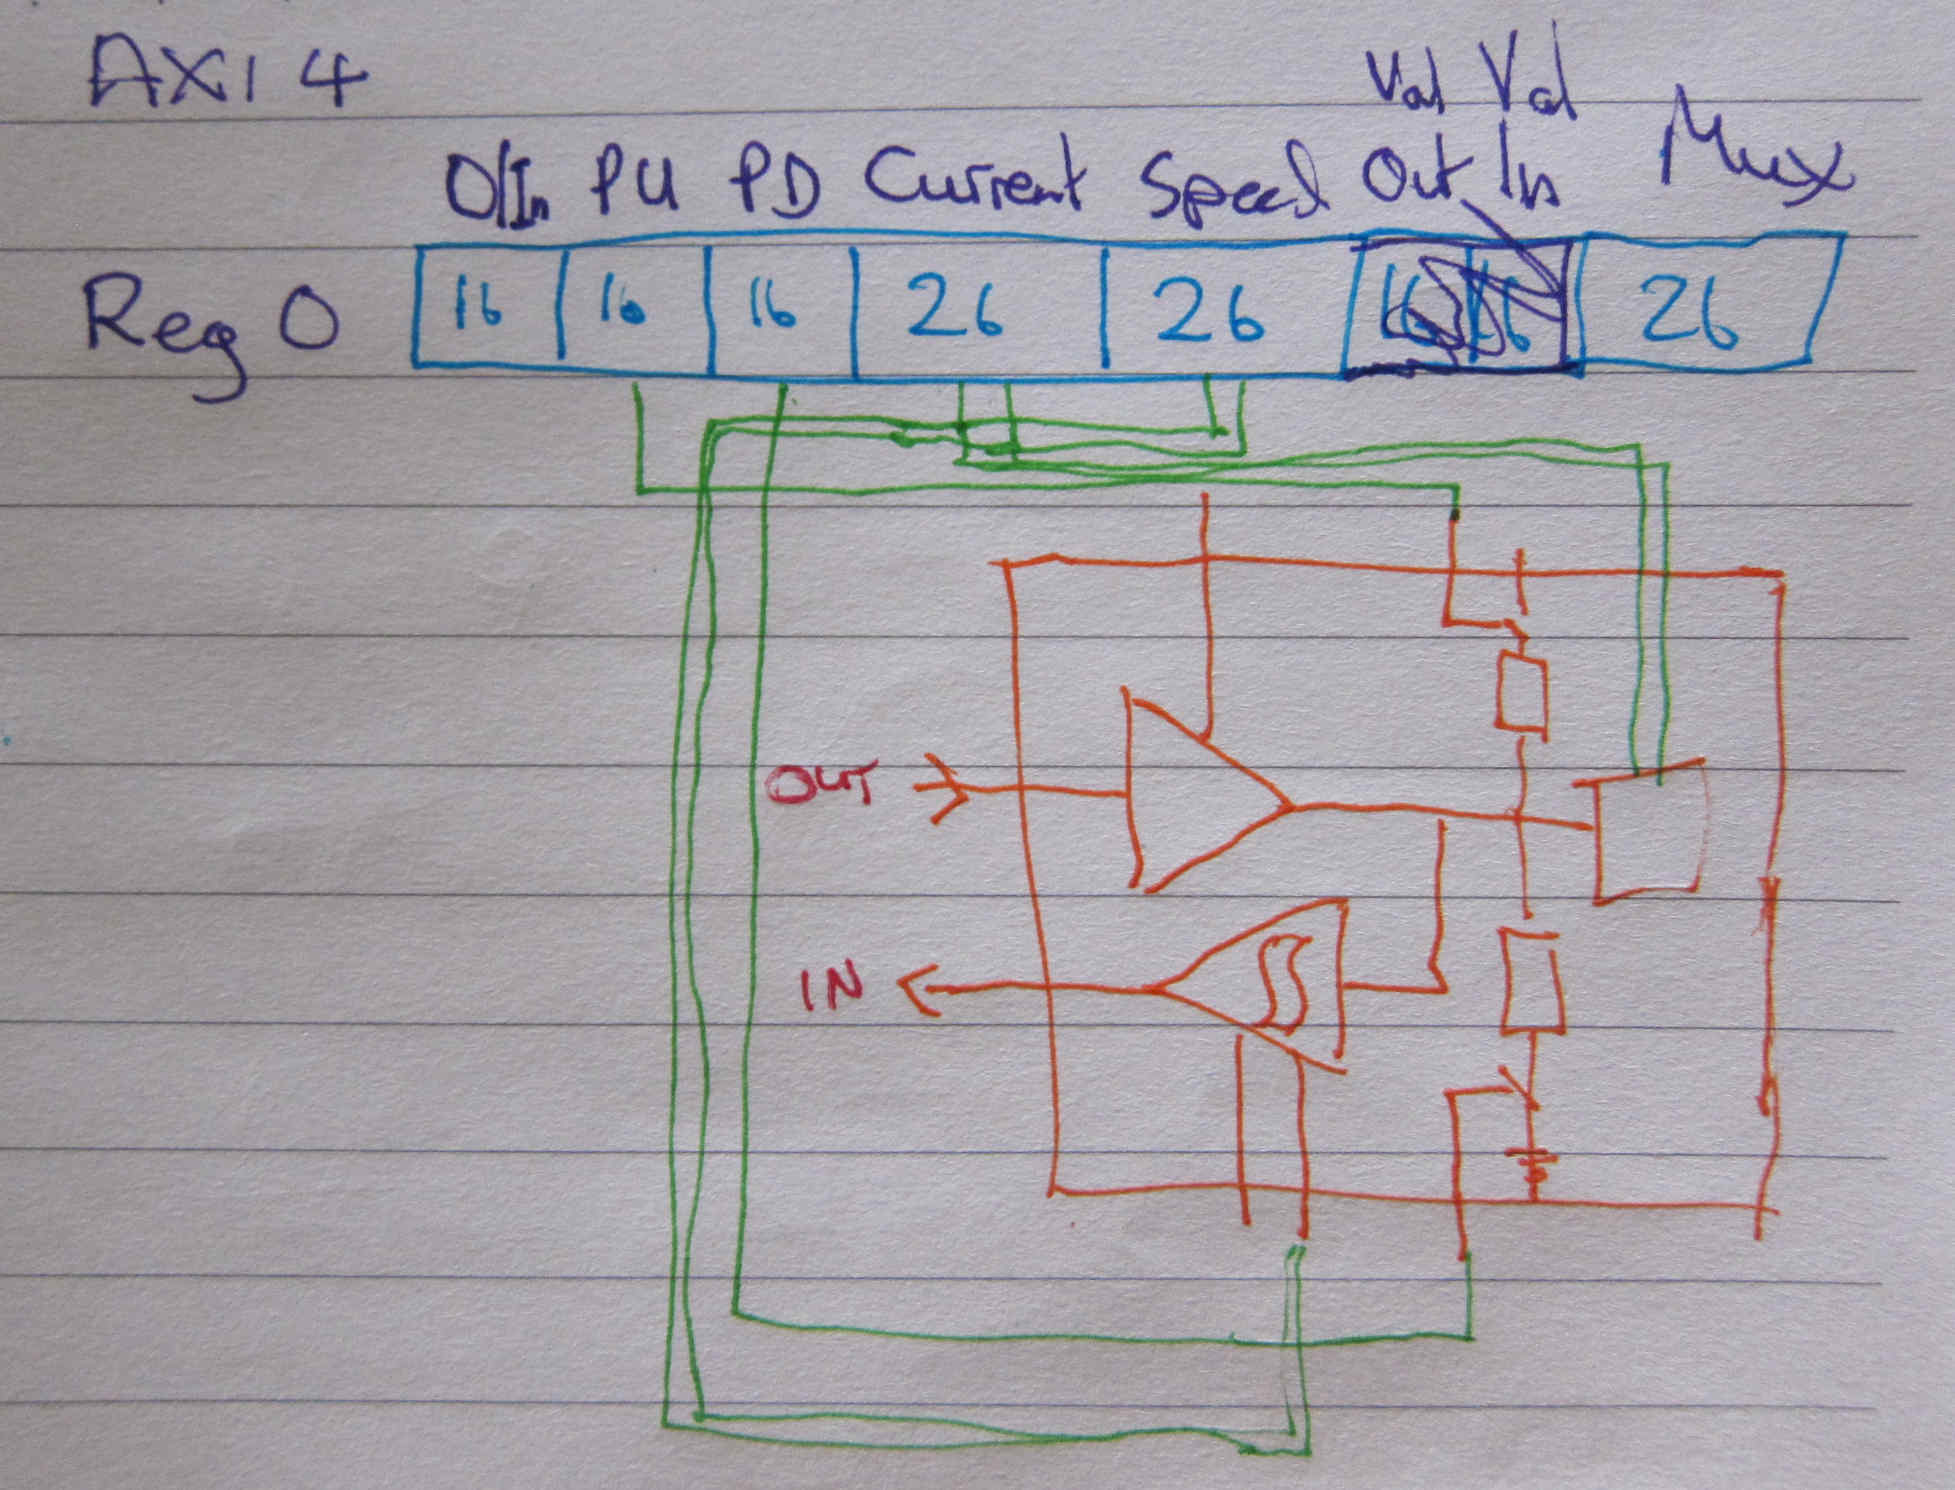
\includegraphics[height=2.5in]{reg_gpio_cap_ctrl.jpg}\\
  {\bf pullup/down, hysteresis, current, edge-detection}
 \end{center}
}


\frame{\frametitle{GPIO (only): Simplified I/O pad Diagram (FN only)}
 \begin{center}
  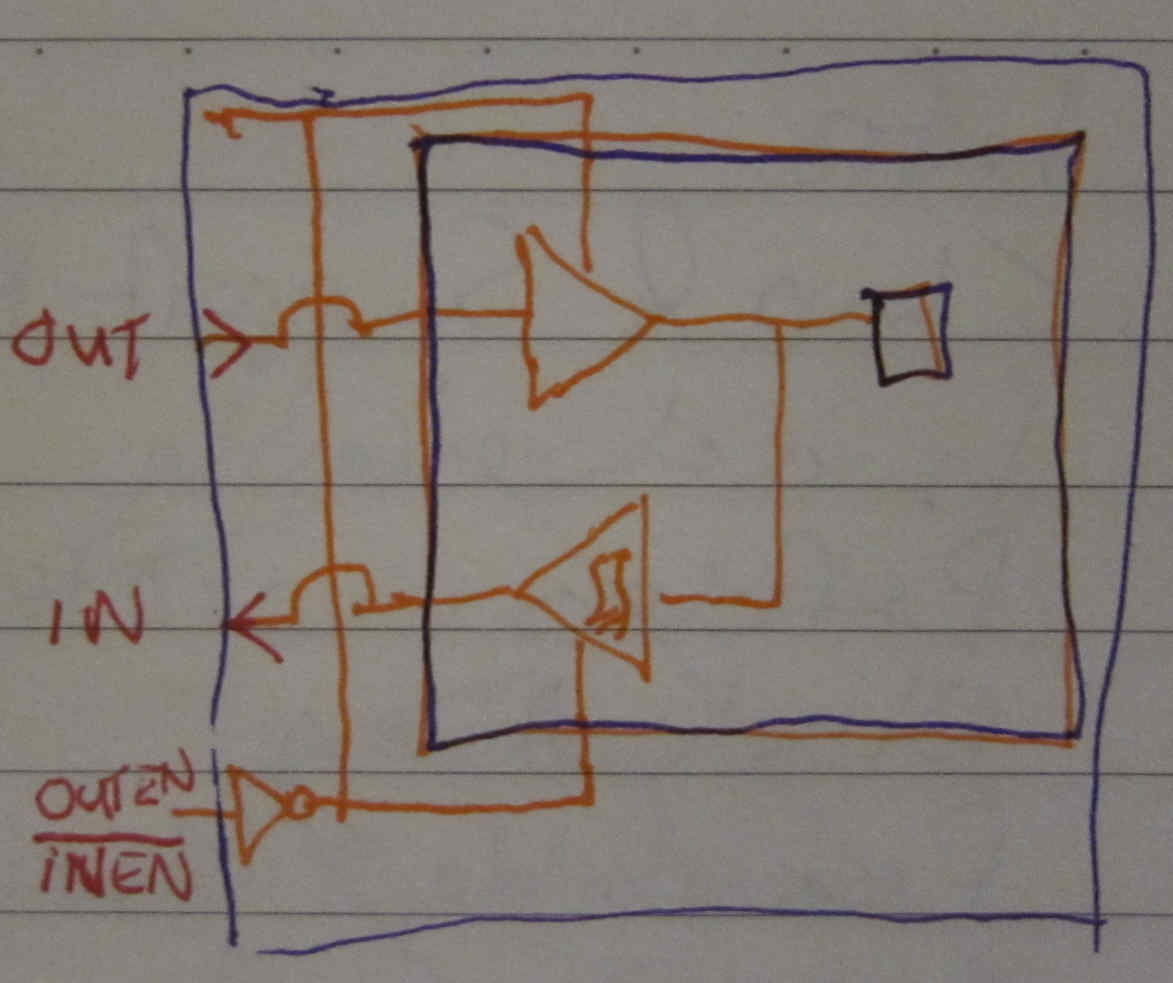
\includegraphics[height=2.5in]{reg_gpio_pinblock.jpg}\\
  {\bf 3 wires: IN, OUT, OUTEN (also = !INEN) }
 \end{center}
}


\frame{\frametitle{Output Muxer (very simple)}
 \begin{center}
  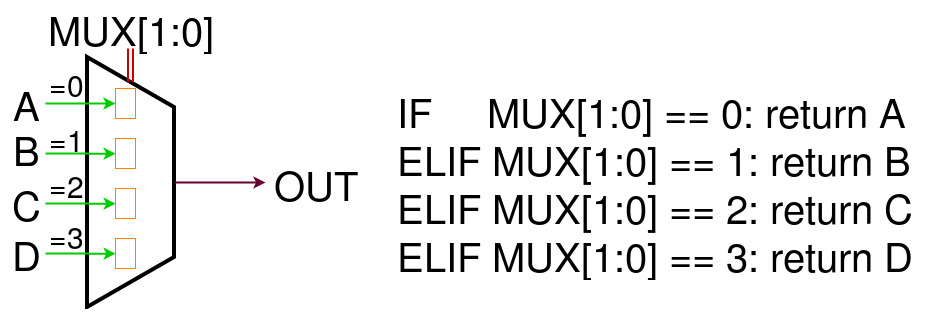
\includegraphics[height=1.1in]{reg_gpio_out_mux.jpg}\\
  {\bf Ouput Muxer using 2-bit address selection}\\
 \end{center}
 \begin{itemize}
   \item Very straightforward (deceptively so, like SRAM cells)
   \item Used in both OUT routing and Direction-control routing\\
	     (same address for each, connected to same FNs)
   \item More complex pinmux will have 3-bit addressing (8 FNs)\\
		 (Note: not all outputs will be connected, depends on pinmux)
 \end{itemize}
}


\frame{\frametitle{In/Out muxing, direction control: GPIO just a FN}
 \begin{center}
  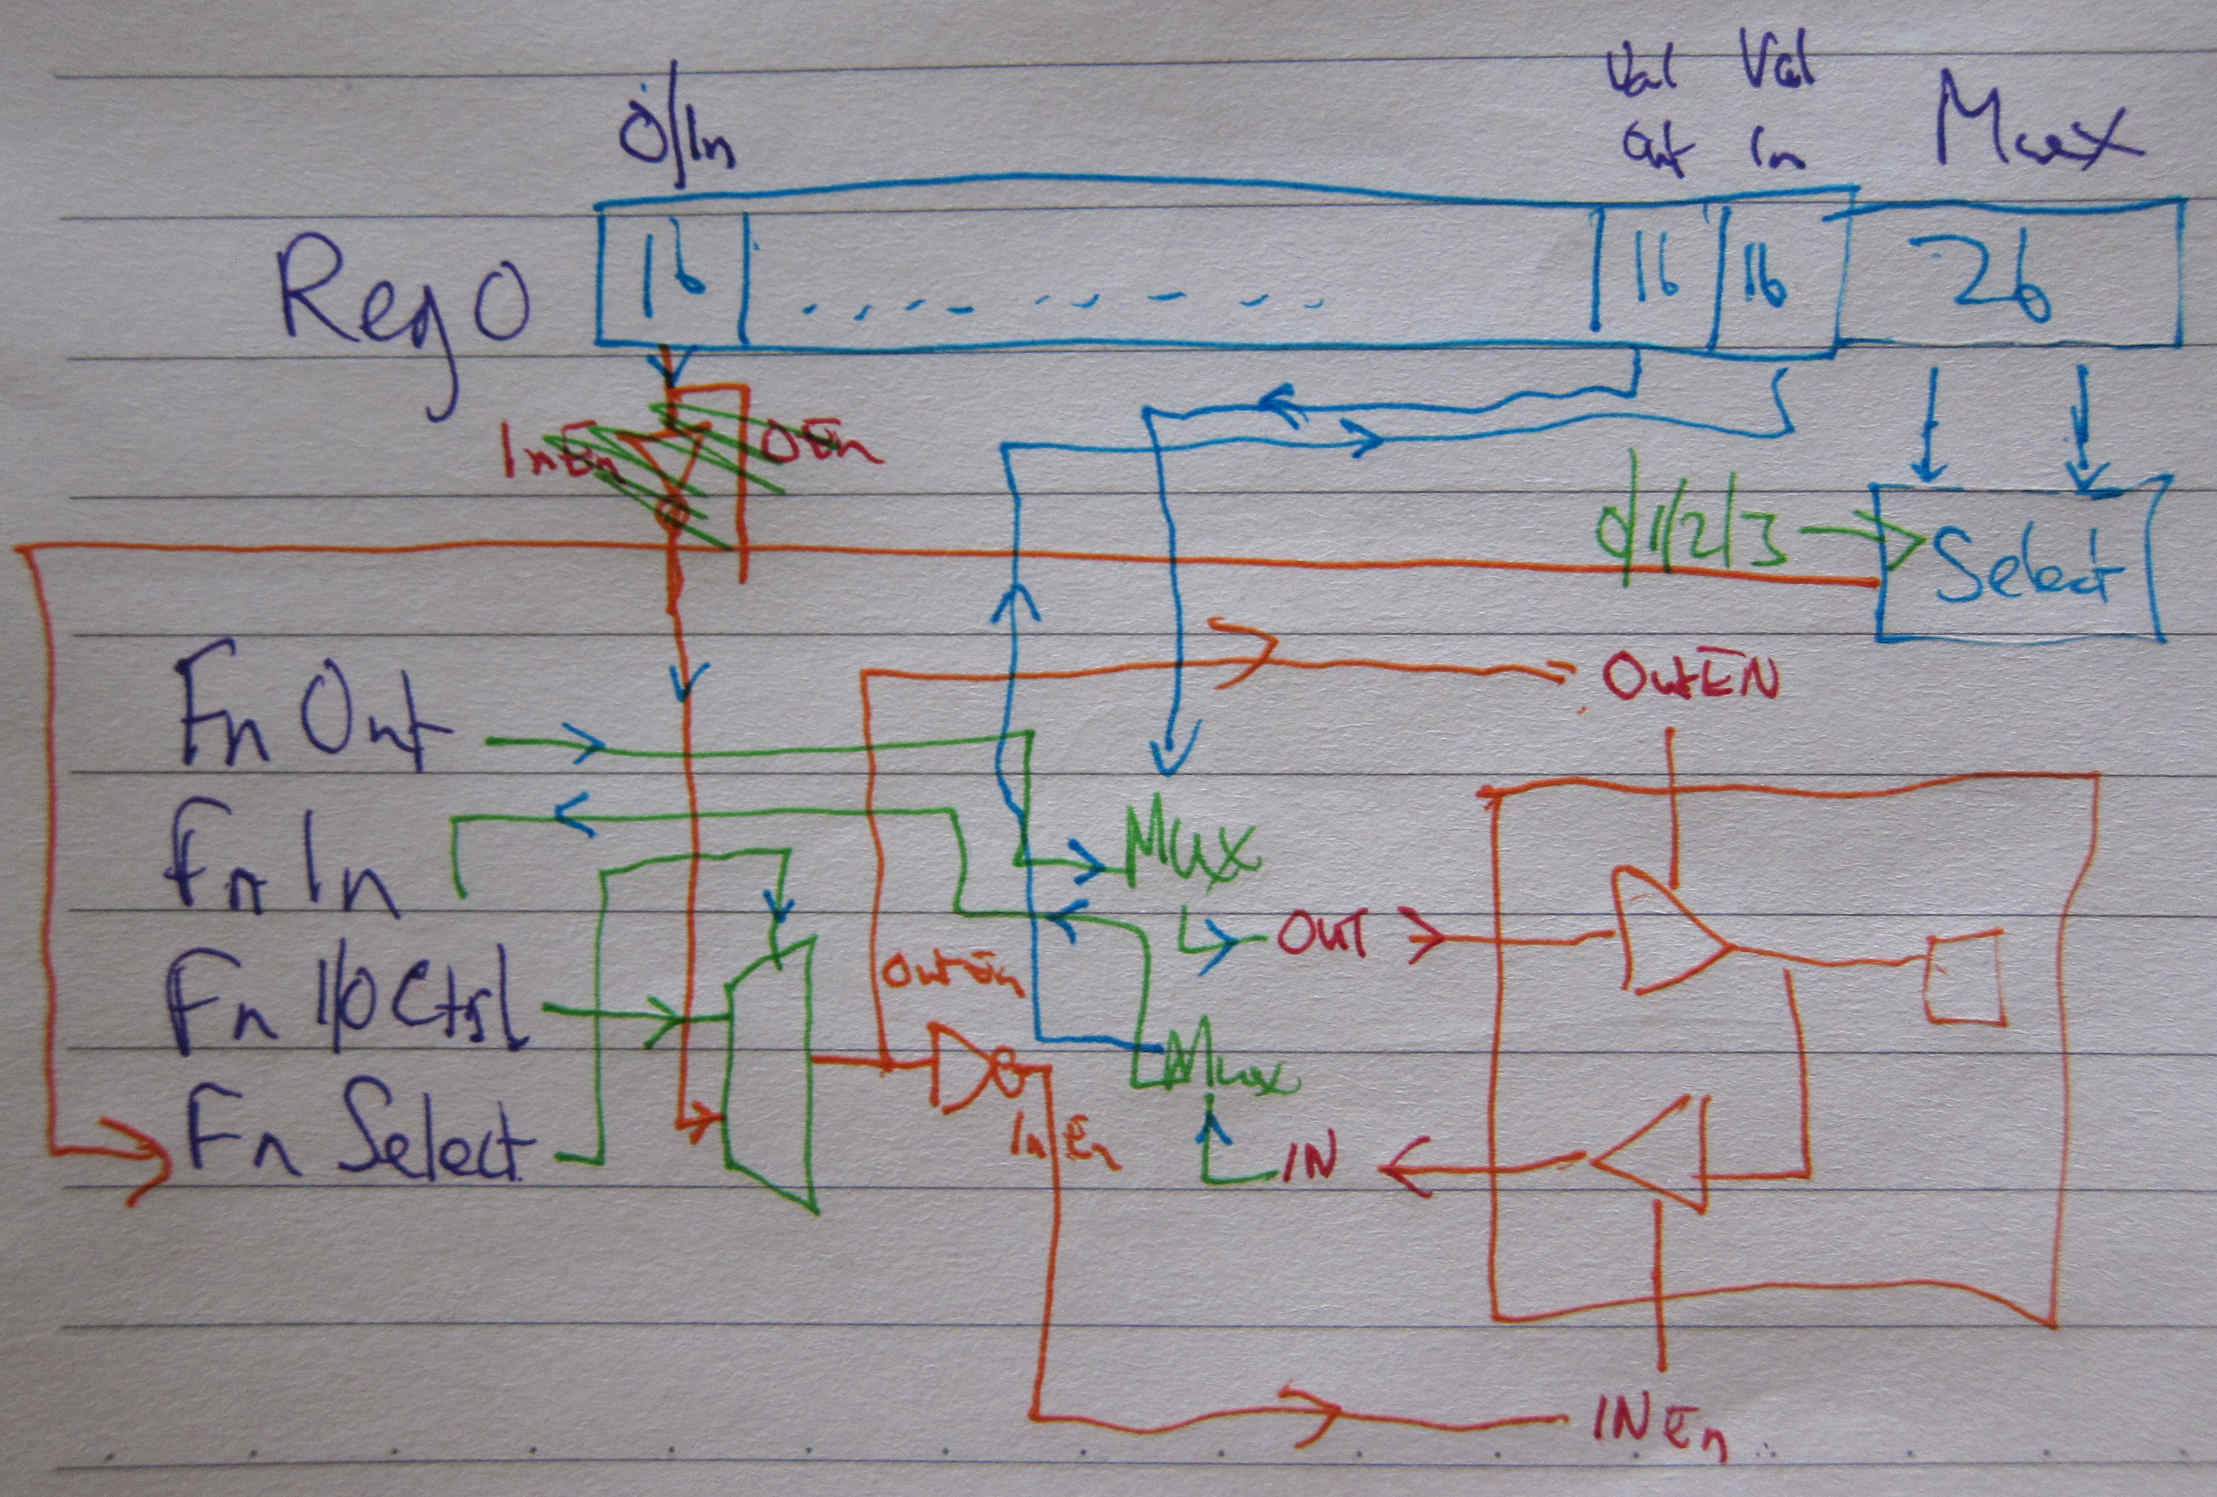
\includegraphics[height=2.5in]{reg_gpio_fn_ctrl.jpg}\\
  {\bf Note: function can control I/O direction (bus)}
 \end{center}
}


\frame{\frametitle{Direction Control: Function not bi-directional (bus)}
 \begin{center}
  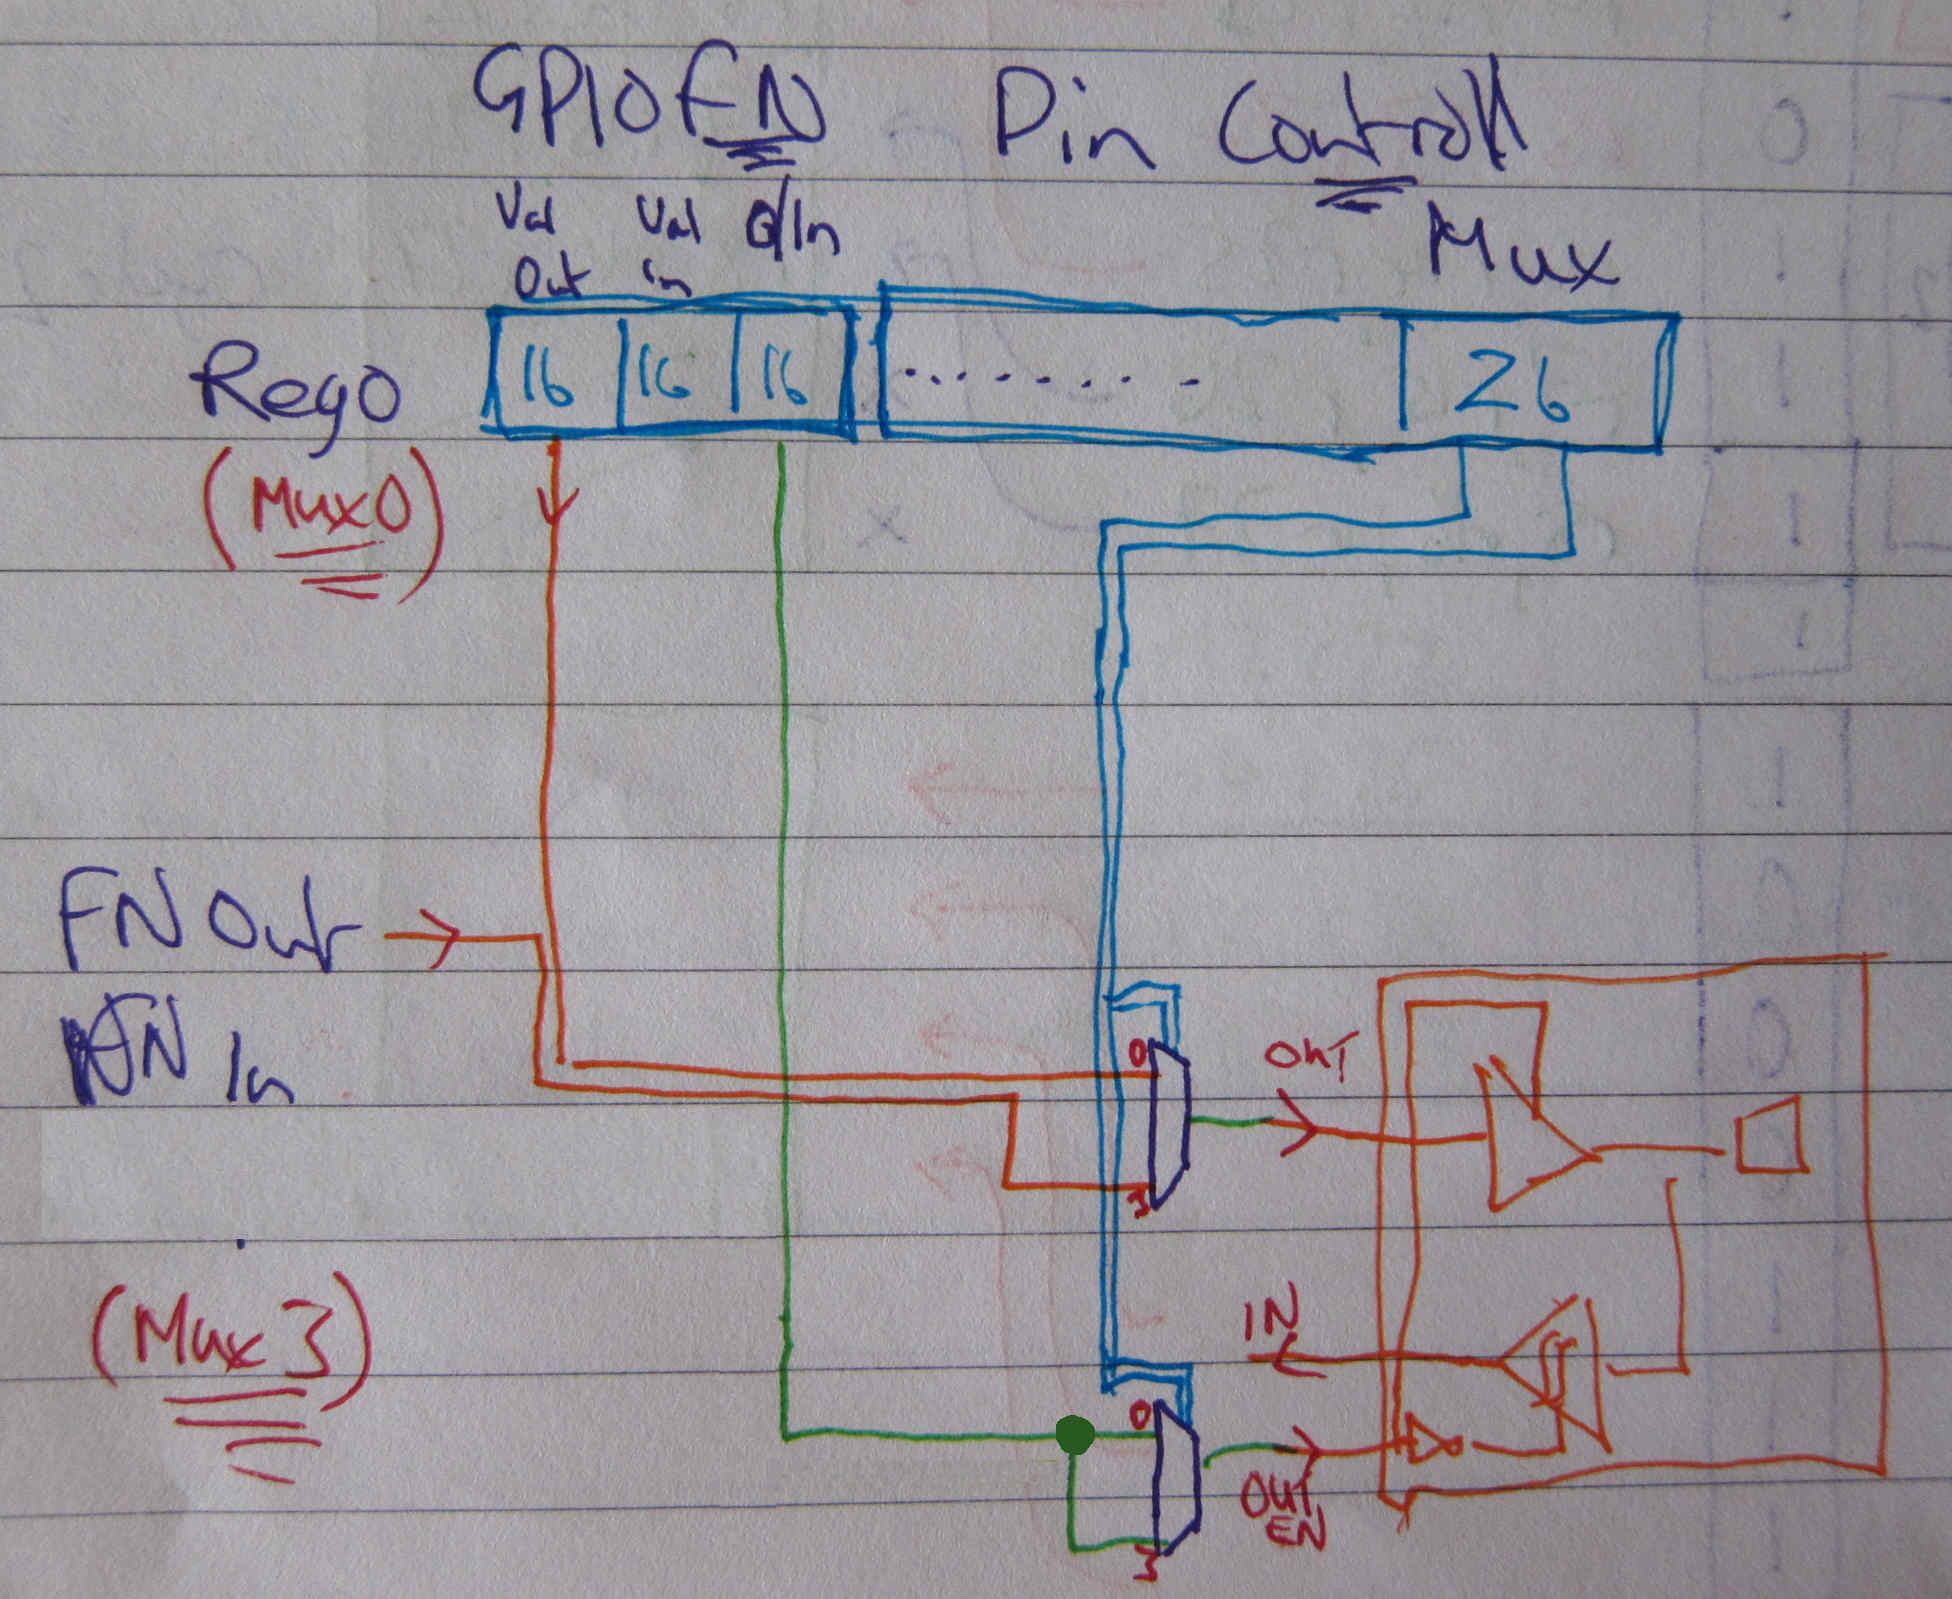
\includegraphics[height=2.5in]{reg_gpio_fn_ctrl2.jpg}\\
  Note: Function {\bf does not} control I/O direction
 \end{center}
}


\frame{\frametitle{Output (and OUTEN) Wiring. 2 pins, 2 GPIO, 2 Fns}
 \begin{center}
  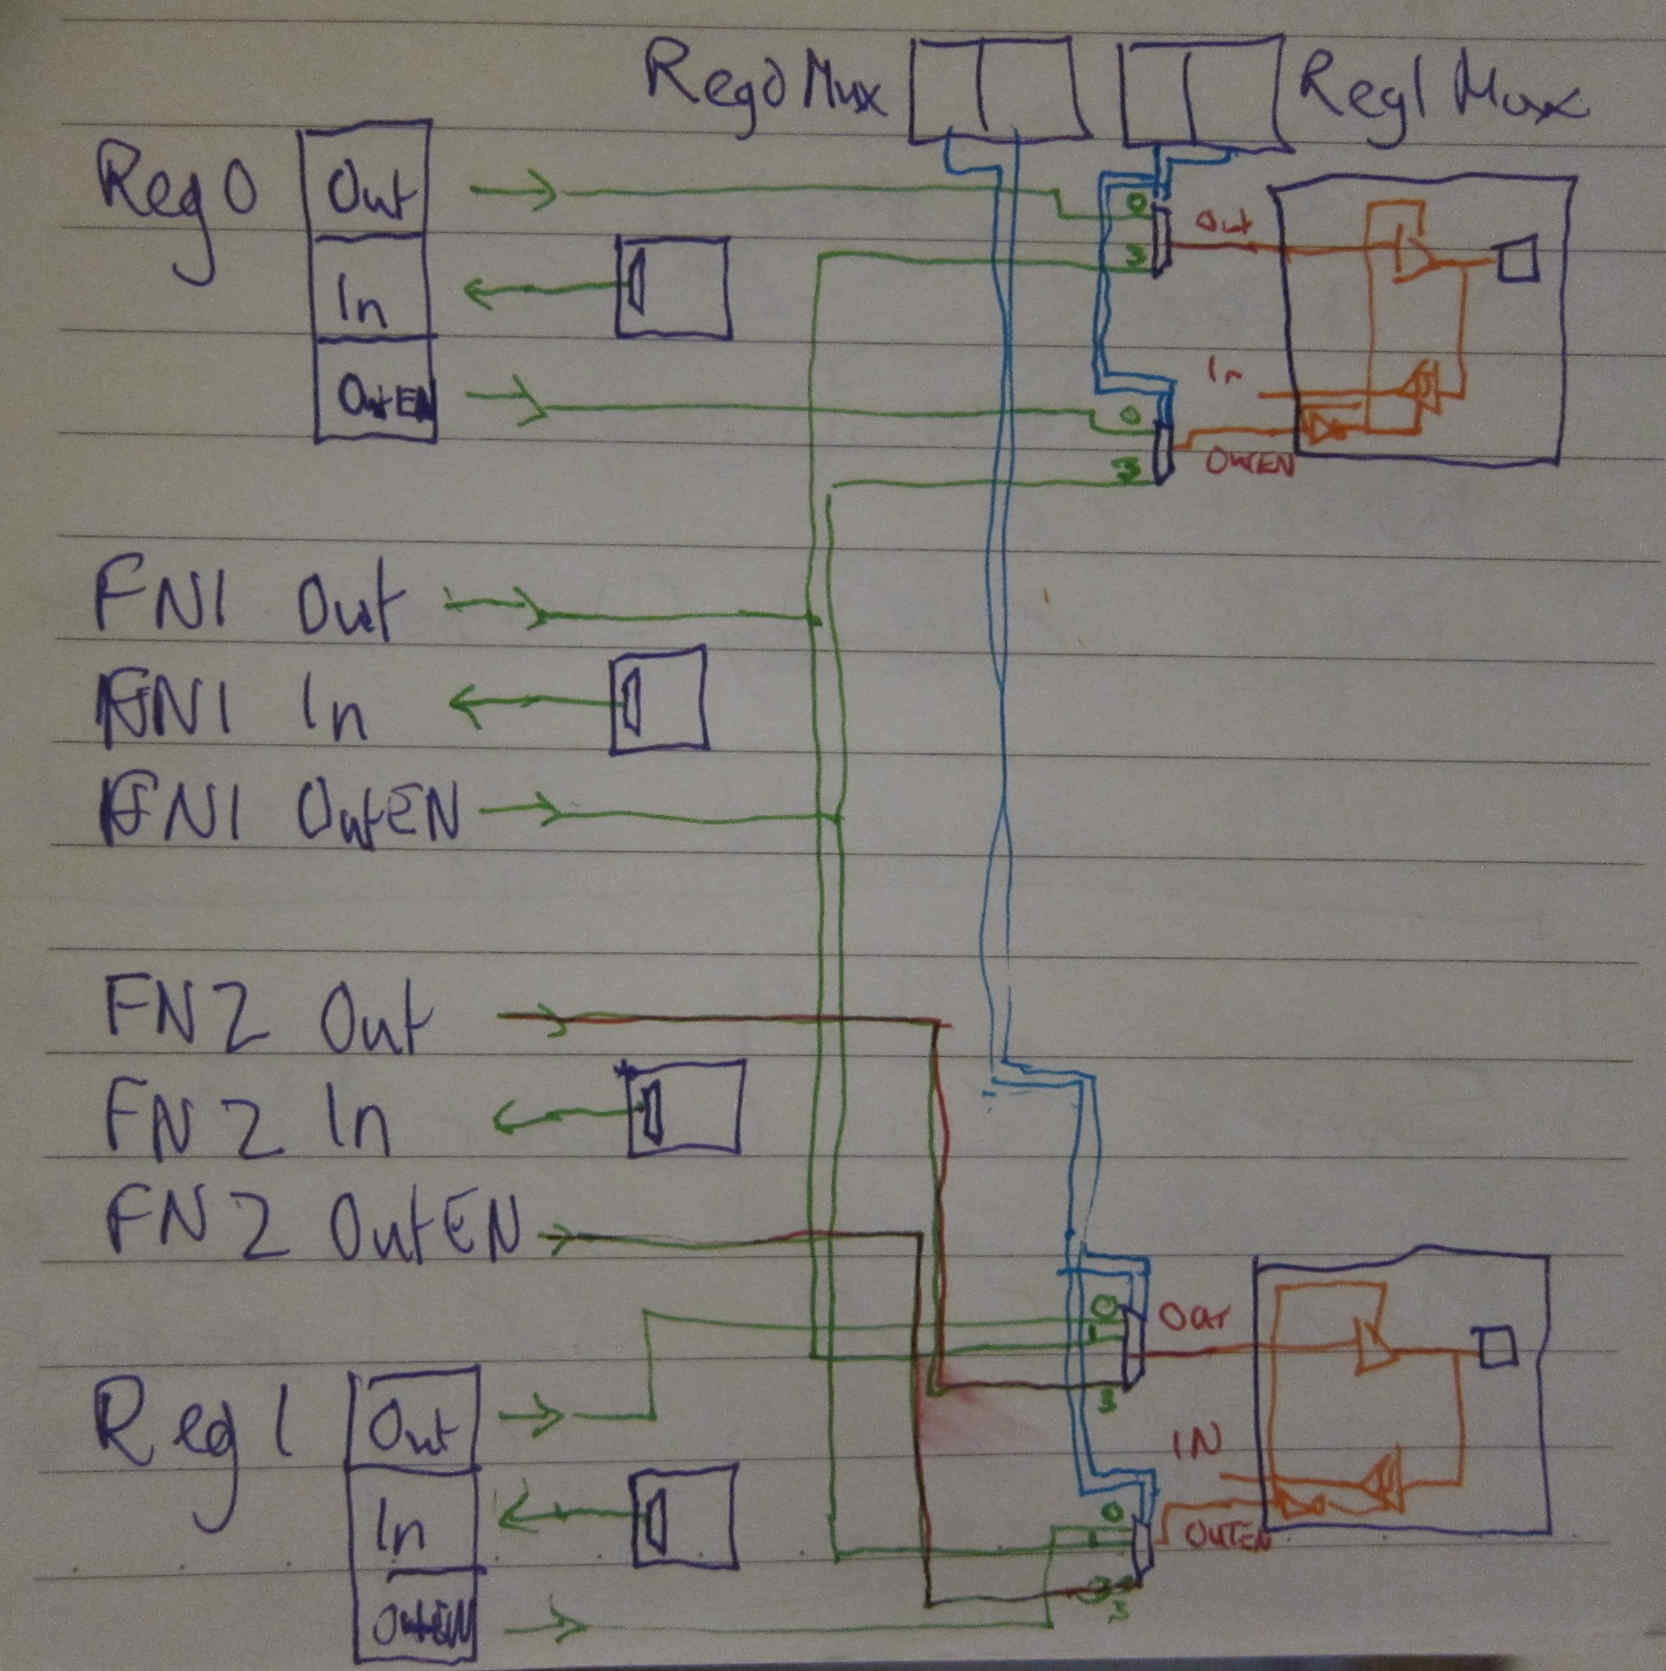
\includegraphics[height=2.5in]{reg_gpio_out_wiring.jpg}\\
  {\bf Reg0 for Pin0, Reg1 for Pin1, Output and OUTEN same mux }
 \end{center}
}


\frame{\frametitle{Input Selection and Priority Muxing}
 \begin{center}
  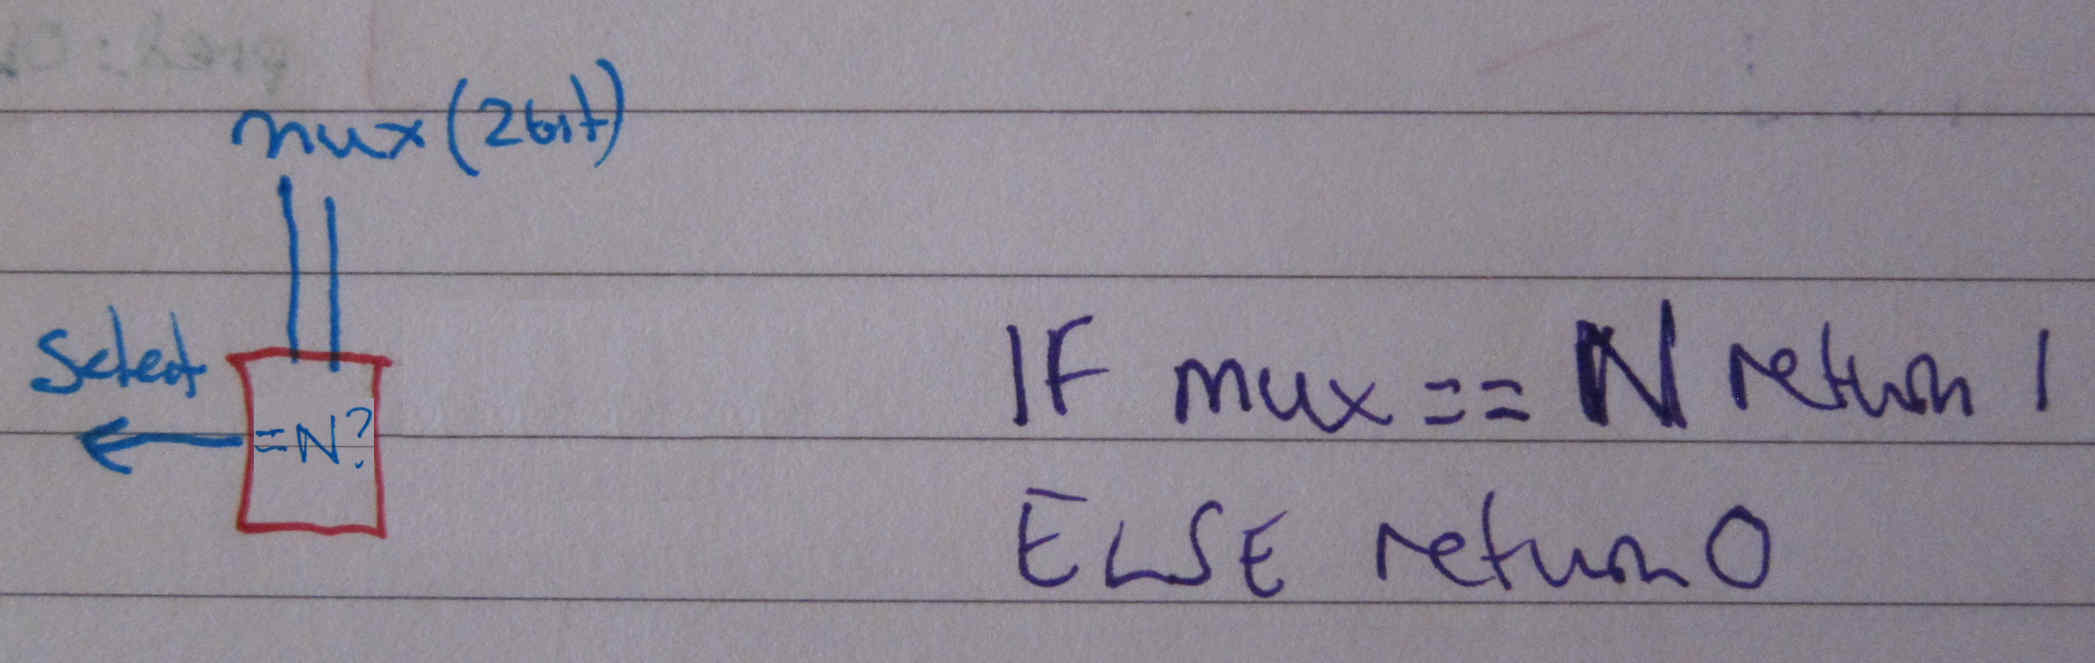
\includegraphics[height=0.75in]{reg_gpio_comparator.jpg}\\
  {\bf Muxer enables input selection}\\
  \vspace{10pt}
  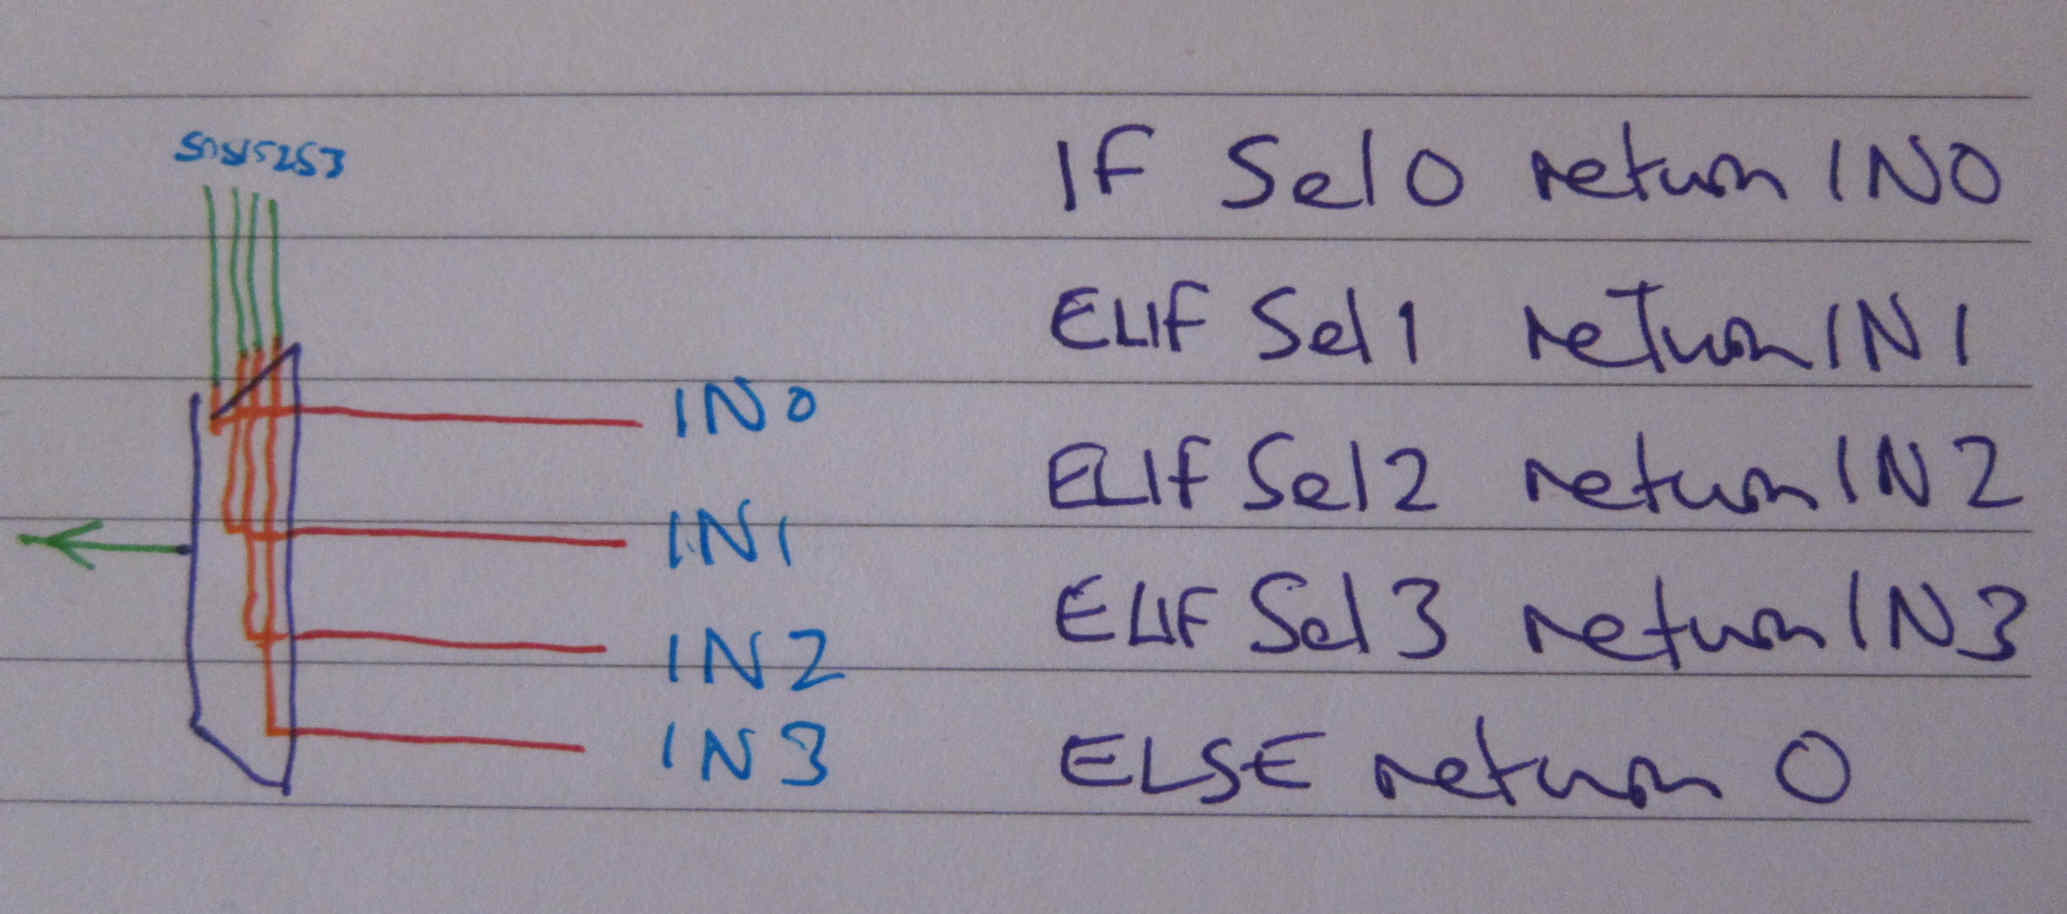
\includegraphics[height=1.25in]{reg_gpio_in_prioritymux.jpg}\\
  {\bf However multiple inputs must be prioritised }
 \end{center}
}


\frame{\frametitle{Input Priority-Mux Wiring: very different from Out-Mux}
 \begin{center}
  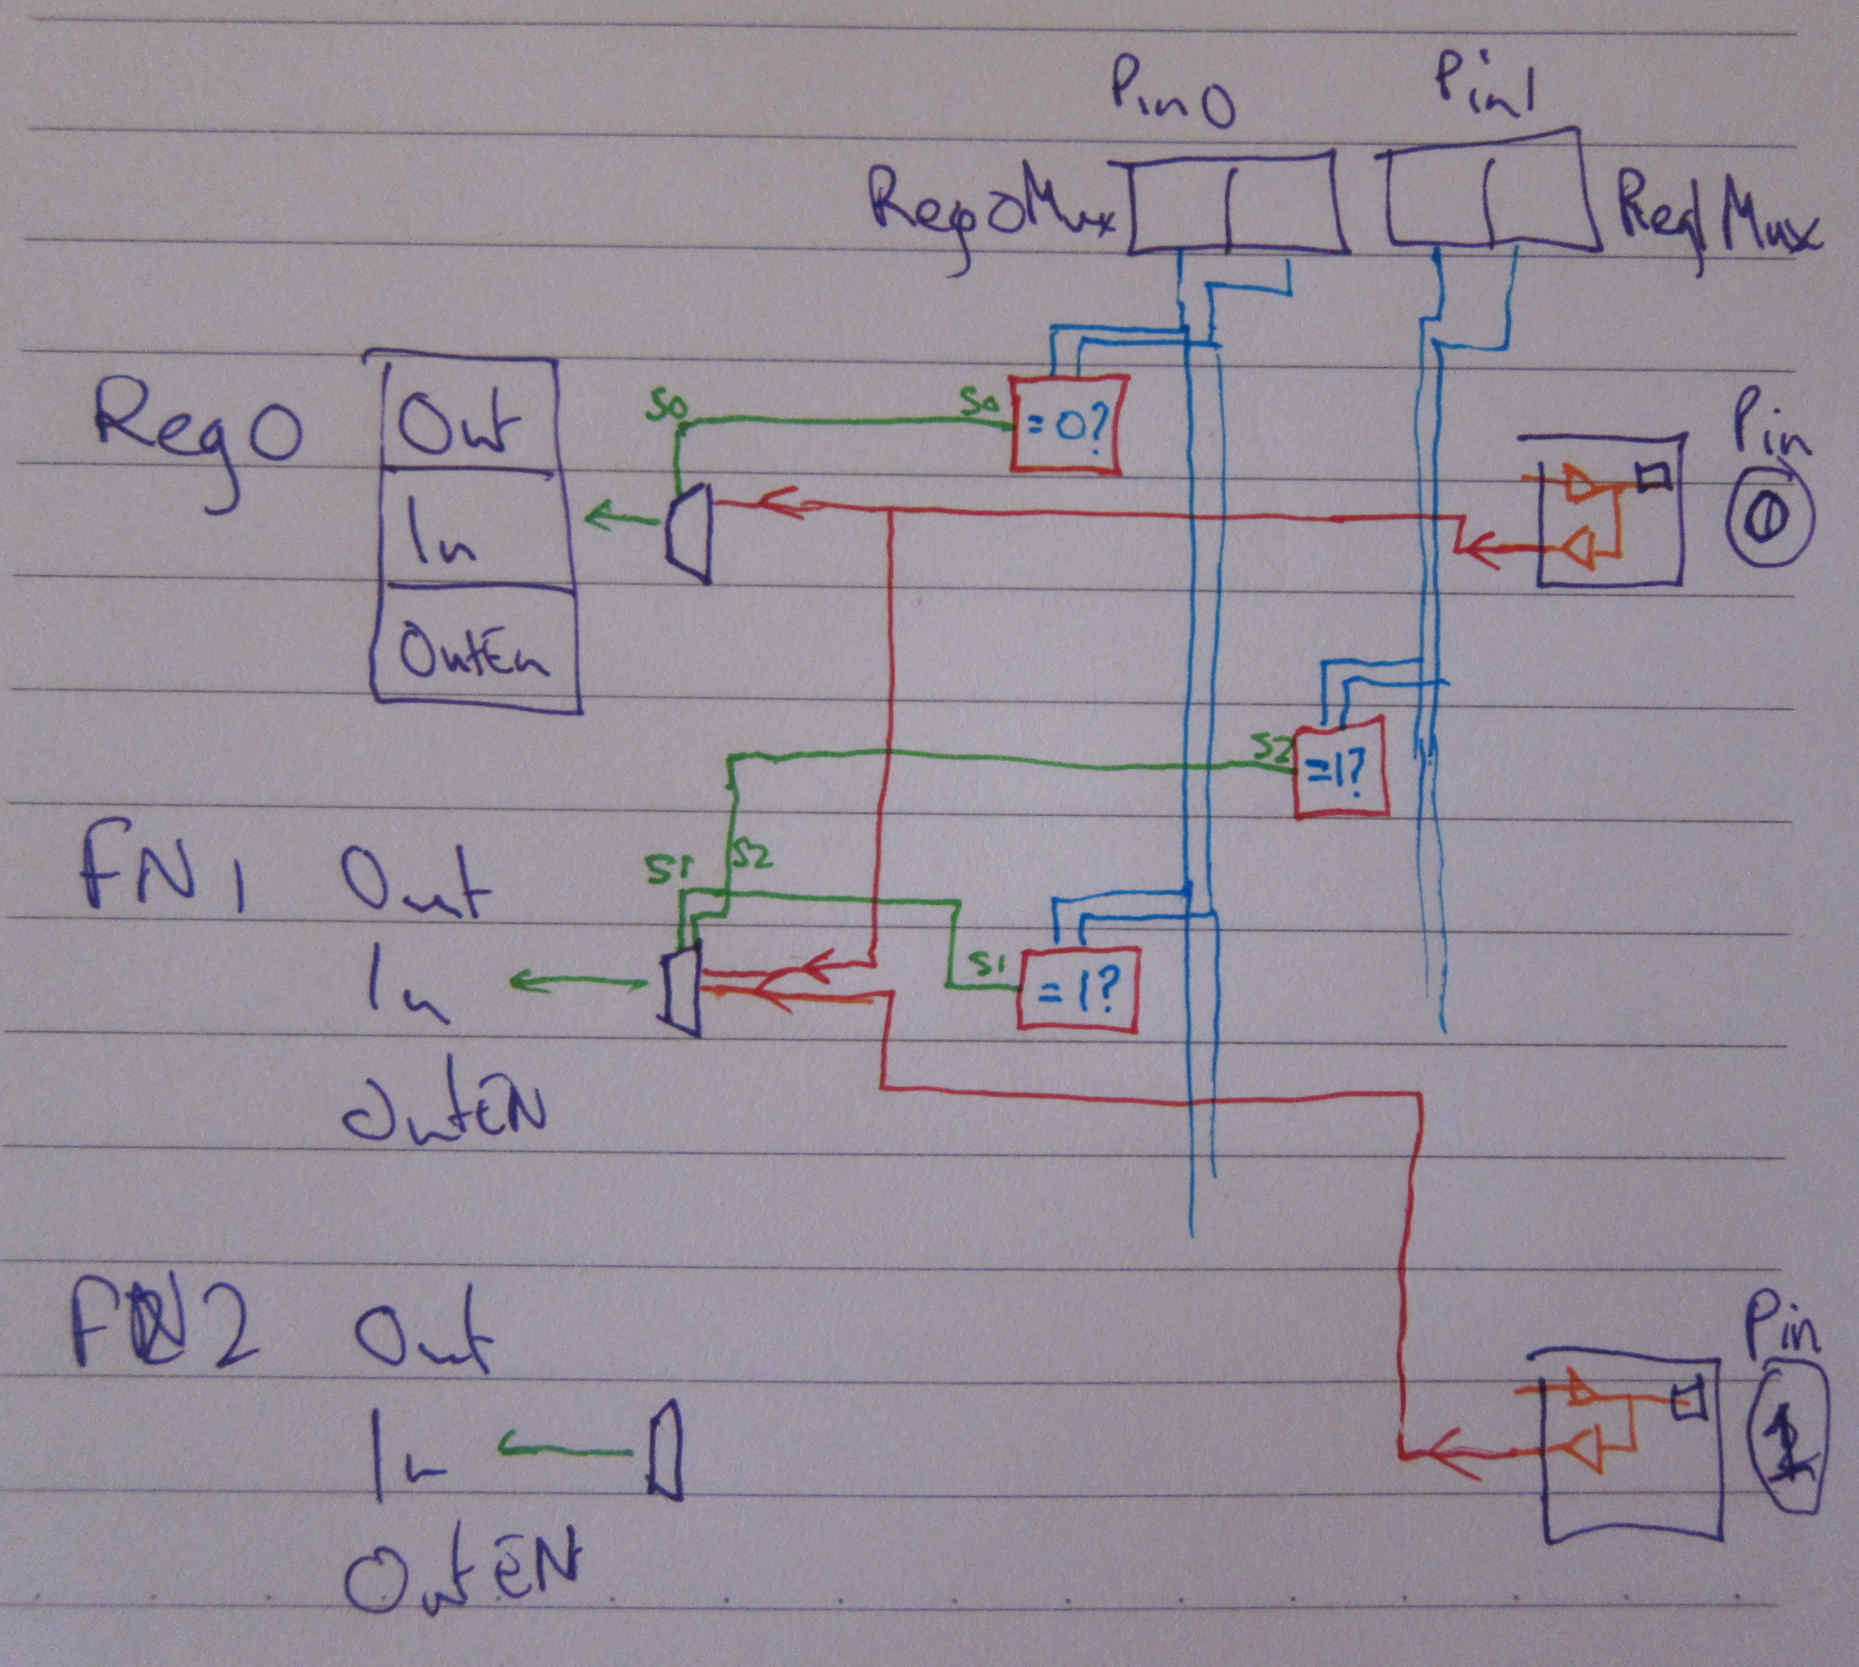
\includegraphics[height=2.5in]{reg_gpio_in_wiring.jpg}\\
  {\bf Pin Mux selection vals NOT same as FN selection vals}
 \end{center}
}


\frame{\frametitle{Input Priority-Mux Wiring}

 \begin{itemize}
   \item In-Muxer selection number (0,1,2,3) obviously has to match
         with Out-Muxer order (otherwise a bi-directional FN
         needs different Mux-register settings for
          selecting either IN or OUT)
	     \vspace{6pt}
   \item Priority-mux selection values do not actually matter,
         and have nothing to do with the actual Muxer settings.
	     \vspace{6pt}
   \item GPIO FN's input muxer is nothing more than an AND gate\\
         (you never route more than one pin to one GPIO)
	     \vspace{6pt}
   \item Any other FN with only 1:1 In also an AND gate \\
	     (this just always happens to be true for GPIO)
	     \vspace{6pt}
   \item Not all FNs have input capability: clearly they will not
	     be included in the In-Muxing. 
  \end{itemize}
}


\frame{\frametitle{Summary}

 \begin{itemize}
   \item TODO
  \end{itemize}
}


\frame{
  \begin{center}
    {\Huge The end\vspace{20pt}\\
		   Thank you\vspace{20pt}\\
		   Questions?\vspace{20pt}
	}
  \end{center}
  
  \begin{itemize}
	\item http://libre-riscv.org/shakti/m\_class/pinmux/
  \end{itemize}
}


\end{document}
